\documentclass[12pt]{article}

\usepackage{fontspec}
\newfontfamily\handwriting{a-casual-handwritten-pen}[Path=../assets/fonts/,Extension=.ttf,Scale=1.5]
\newfontfamily\comic{Comic Neue}

\usepackage[utf8]{inputenc}
\usepackage{amsmath}
\usepackage{amssymb}
\usepackage{enumitem}
\usepackage{xcolor}
\usepackage{soul}
\usepackage{tikz}
\usepackage[most]{tcolorbox}
\usepackage{titlesec}
\usepackage{multicol}
\usepackage{environ}

\usetikzlibrary{fit, positioning, arrows.meta, decorations.pathreplacing}

% --- Custom Colors ---
\definecolor{primaryblue}{RGB}{42, 111, 151}
\definecolor{exbg}{RGB}{255, 240, 245}
\definecolor{rulebg}{RGB}{232, 245, 233}
\definecolor{highlight}{RGB}{255, 243, 176}
\definecolor{pinkanno}{RGB}{255, 105, 180}
\definecolor{purpleanno}{RGB}{147, 112, 219}
\definecolor{solutionbg}{RGB}{245, 245, 255}

% --- Header Styling ---
\titleformat{\section}{\color{primaryblue}\normalfont\Large\bfseries}{\thesection}{1em}{}
\titleformat{\subsection}{\color{primaryblue}\normalfont\large\bfseries}{\thesubsection}{1em}{}

% --- Friendly Boxes ---
% --- Auto-numbered Example Box ---
\newcounter{examplenum}

\newtcolorbox{friendlyexbox}[1]{
    colback=exbg,
    colframe=pinkanno!50,
    arc=5pt,
    title=\textbf{#1},
    coltitle=black,
    attach title to upper,
    after title={:\quad}
}

\newenvironment{friendlyex}{%
    \refstepcounter{examplenum}%
    \begin{friendlyexbox}{Example \theexamplenum}%
}{%
    \end{friendlyexbox}%
}

\newtcolorbox{friendlyrule}[1]{
    colback=rulebg,
    colframe=primaryblue!30,
    arc=5pt,
    fonttitle=\bfseries,
    title={#1},
    coltitle=primaryblue
}

\newcommand{\funhl}[1]{\sethlcolor{highlight}\hl{#1}}

% --- Show/Hide Solutions ---
\newif\ifshowsolutions

% Uncomment the next line to show solutions.
\showsolutionstrue

\newcommand{\solutionblank}{\vspace{25ex}}

\NewEnviron{solutionbox}{
\ifshowsolutions
\begin{tcolorbox}[
    colback=solutionbg,
    colframe=purpleanno!45,
    arc=5pt,
    title={Solution},
    coltitle=primaryblue,
    fonttitle=\bfseries
]
\BODY
\end{tcolorbox}
\else
\solutionblank
\fi
}

\begin{document}
\handwriting

\begin{center}
    \Large\textbf{\color{primaryblue}Module 2 Lesson 4\\Algebra of Functions and Function Composition} \\
    \vspace{0.2cm}
    \hrule
\end{center}

\section*{Objectives}

\begin{friendlyrule}{In this lesson, we will learn how to}
\begin{itemize}
    \item find the sum, difference, product, and quotient of two functions;
    \item determine the domain of combined functions;
    \item find and evaluate the composition of two functions;
    \item distinguish $(f\circ g)(x)$ from $(fg)(x)$.
\end{itemize}
\end{friendlyrule}

\section*{1. Sum, Difference, Product, and Quotient of Functions}

\begin{friendlyrule}{Algebra of Functions}
If $f(x)$ and $g(x)$ are functions, then for all $x$ common to the domains of both functions:
\begin{enumerate}[label=\arabic*.]
    \item Sum: $(f+g)(x)=f(x)+g(x)$
    \item Difference: $(f-g)(x)=f(x)-g(x)$
    \item Product: $(fg)(x)=f(x)\cdot g(x)$
    \item Quotient: $\left(\dfrac{f}{g}\right)(x)=\dfrac{f(x)}{g(x)}$, provided $g(x)\neq 0$.
\end{enumerate}
\end{friendlyrule}

\begin{friendlyex}{}
If $f(x)=x^2+1$ and $g(x)=3x-5$, find the following and give the domain in interval notation.
\begin{itemize}
    \item[(a)] $(f+g)(x)$
    \item[(b)] $(f+g)(3)$
    \item[(c)] $(fg)(x)$
    \item[(d)] $(fg)(4)$
    \item[(e)] $(f-g)(x)$
    \item[(f)] $(f-g)(-2)$
    \item[(g)] $\left(\dfrac{f}{g}\right)(x)$
\end{itemize}
\end{friendlyex}

 

\begin{solutionbox}
\textbf{(a)}

\[
(f+g)(x)=(x^2+1)+(3x-5)=x^2+3x-4.
\]

Both $f$ and $g$ are polynomials, so the domain is $(-\infty,\infty)$.

\textbf{(b)}

\[
(f+g)(3)=9+3(3)-4=9+9-4=14.
\]

\textbf{(c)}

\[
(fg)(x)=(x^2+1)(3x-5)=3x^3-5x^2+3x-5.
\]

Domain: $(-\infty,\infty)$.

\textbf{(d)}

\[
(fg)(4)=(16+1)(12-5)=17\cdot 7=119.
\]

\textbf{(e)}

\[
(f-g)(x)=(x^2+1)-(3x-5)=x^2-3x+6.
\]

Domain: $(-\infty,\infty)$.

\textbf{(f)}

\[
(f-g)(-2)=4-3(-2)+6=4+6+6=16.
\]

\textbf{(g)}

\[
\left(\frac{f}{g}\right)(x)=\frac{x^2+1}{3x-5}.
\]

We need $3x-5\neq 0$, i.e., $x\neq\dfrac53$. Domain: $\left(-\infty,\dfrac53\right)\cup\left(\dfrac53,\infty\right)$.
\end{solutionbox}

  

\begin{friendlyex}{}
If $f(x)=x^2-5$ and $g(x)=\sqrt{6-x}$, find $(fg)(x)$ and give the domain in interval notation.
\end{friendlyex}

 

\begin{solutionbox}
\[
(fg)(x)=(x^2-5)\sqrt{6-x}.
\]

$f$ has domain $(-\infty,\infty)$. For $g$, we need $6-x\ge 0$, i.e., $x\le 6$. The combined domain is

\[
(-\infty,6].
\]
\end{solutionbox}

  

\begin{friendlyex}{}
Use the graph of $f$ and $g$ below to determine the following:
\begin{itemize}
    \item[(a)] $(f+g)(-6)$
    \item[(b)] $(f-g)(-2)$
    \item[(c)] $(f\cdot g)(3)$
    \item[(d)] $\left(\dfrac{f}{g}\right)(-2)$
\end{itemize}
\end{friendlyex}

\begin{center}
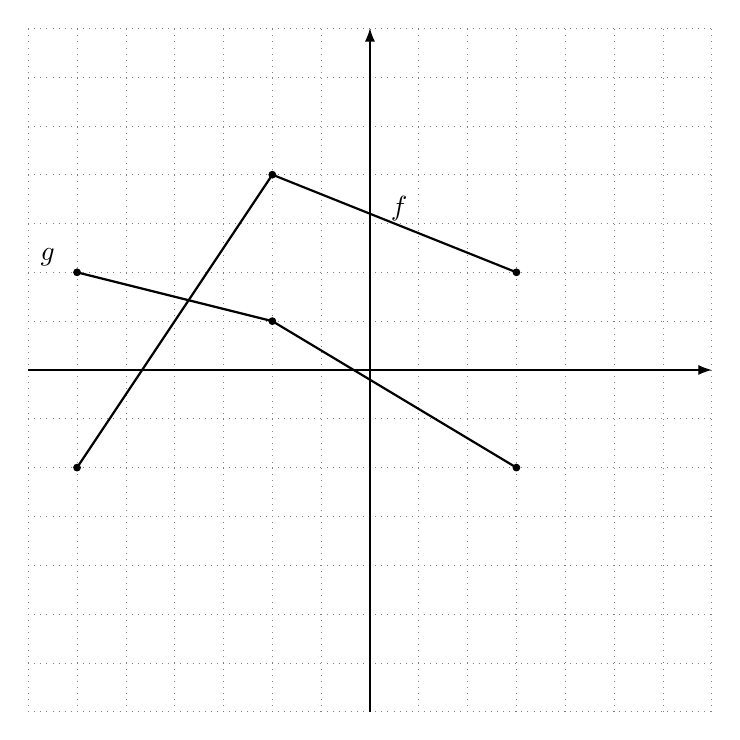
\begin{tikzpicture}[scale=0.62]
\draw[help lines, dotted] (-7,-7) grid (7,7);
\draw[-{Latex}] (-7,0) -- (7,0);
\draw[-{Latex}] (0,-7) -- (0,7);
% f: tent shape through (-6,-2),(-2,4),(3,2)
\draw[thick] (-6,-2) -- (-2,4) -- (3,2);
\fill (-6,-2) circle (0.08);
\fill (-2,4) circle (0.08);
\fill (3,2) circle (0.08);
\node at (0.6,3.3) {$f$};
% g: gently declining through (-6,2),(-2,1),(3,-2)
\draw[thick] (-6,2) -- (-2,1) -- (3,-2);
\fill (-6,2) circle (0.08);
\fill (-2,1) circle (0.08);
\fill (3,-2) circle (0.08);
\node at (-6.6,2.3) {$g$};
\end{tikzpicture}
\end{center}

 

\begin{solutionbox}
From the graph: $f(-6)=-2$, $f(-2)=4$, $f(3)=2$, and $g(-6)=2$, $g(-2)=1$, $g(3)=-2$.

\textbf{(a)}

\[
(f+g)(-6)=f(-6)+g(-6)=-2+2=0.
\]

\textbf{(b)}

\[
(f-g)(-2)=f(-2)-g(-2)=4-1=3.
\]

\textbf{(c)}

\[
(f\cdot g)(3)=f(3)\cdot g(3)=2\cdot(-2)=-4.
\]

\textbf{(d)}

\[
\left(\frac{f}{g}\right)(-2)=\frac{f(-2)}{g(-2)}=\frac{4}{1}=4.
\]
\end{solutionbox}

  

\section*{2. Composition of Functions}

Composing two functions is like connecting two machines that work one after the other: the output of the first machine becomes the input of the second.

\begin{center}
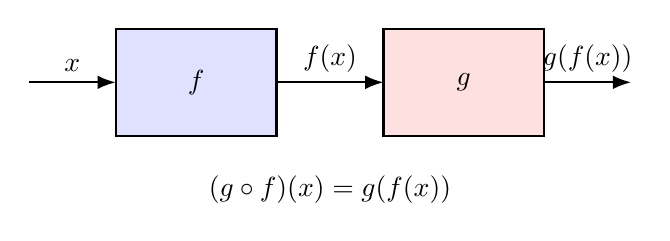
\begin{tikzpicture}[scale=0.85]
\draw[fill=blue!12, thick] (0,0) rectangle (2.4,1.6);
\node at (1.2,0.8) {$f$};
\draw[fill=red!12, thick] (4,0) rectangle (6.4,1.6);
\node at (5.2,0.8) {$g$};
\draw[-{Latex}, thick] (-1.3,0.8) -- (0,0.8) node[midway, above] {$x$};
\draw[-{Latex}, thick] (2.4,0.8) -- (4,0.8) node[midway, above] {$f(x)$};
\draw[-{Latex}, thick] (6.4,0.8) -- (7.7,0.8) node[midway, above] {$g(f(x))$};
\node at (3.2,-0.8) {$(g\circ f)(x)=g(f(x))$};
\end{tikzpicture}
\end{center}

\begin{friendlyrule}{Composition Notation}
If we first apply $f$ to an input $x$, and then apply $g$ to the result, we write the composition as
\[
(g\circ f)(x)=g(f(x)).
\]
The order matters: $g(f(x))$ means $f$ acts first and $g$ acts second.
\begin{itemize}
    \item $g(f(x))$: apply $f$'s formula first, then apply $g$'s formula to the result.
    \item $f(g(x))$: apply $g$'s formula first, then apply $f$'s formula to the result.
\end{itemize}
\end{friendlyrule}

\begin{friendlyrule}{Important Distinction}
$(f\circ g)(x)$ and $(fg)(x)$ are \textbf{different} functions: $(f\circ g)(x)$ is the composition, while $(fg)(x)$ is the product of $f(x)$ and $g(x)$. That is,

\[
f\circ g\ \neq\ fg.
\]
\end{friendlyrule}

\begin{friendlyex}{}
Given $f(x)=3x+4$ and $g(x)=\dfrac{1}{x-1}$, find the following and write the domain in interval notation.
\begin{itemize}
    \item[(a)] $(f\circ g)(x)$
    \item[(b)] $(g\circ f)(x)$
\end{itemize}
\end{friendlyex}

 

\begin{solutionbox}
\textbf{(a)}

\[
(f\circ g)(x)=f(g(x))=3\left(\frac{1}{x-1}\right)+4=\frac{3}{x-1}+4=\frac{3+4(x-1)}{x-1}=\frac{4x-1}{x-1}.
\]

We need $x\neq 1$. Domain: $(-\infty,1)\cup(1,\infty)$.

\textbf{(b)}

\[
(g\circ f)(x)=g(f(x))=\frac{1}{(3x+4)-1}=\frac{1}{3x+3}=\frac{1}{3(x+1)}.
\]

We need $x\neq -1$. Domain: $(-\infty,-1)\cup(-1,\infty)$.
\end{solutionbox}

  

\begin{friendlyex}{}
$f(x)=4-x$ and $g(x)=2x+1$, find:
\begin{itemize}
    \item[(a)] $g(f(1))$
    \item[(b)] $f(g(3))$
    \item[(c)] Compute $f(g(2))$ and $g(f(2))$. Are the two values equal?
\end{itemize}
\end{friendlyex}

 

\begin{solutionbox}
\textbf{(a)} $f(1)=4-1=3$, so $g(f(1))=g(3)=2(3)+1=7$.

\textbf{(b)} $g(3)=2(3)+1=7$, so $f(g(3))=f(7)=4-7=-3$.

\textbf{(c)} $g(2)=2(2)+1=5$, so $f(g(2))=f(5)=4-5=-1$.

$f(2)=4-2=2$, so $g(f(2))=g(2)=2(2)+1=5$.

Since $-1\neq 5$, the two values are \textbf{not} equal --- in general, $f\circ g\neq g\circ f$.
\end{solutionbox}

  

\begin{friendlyex}{}
Use the graph of $f$ and $g$ below to compute the following.
\begin{itemize}
    \item[(a)] $(g\circ f)(-6)$
    \item[(b)] $(f\circ g)(3)$
\end{itemize}
\end{friendlyex}

\begin{center}
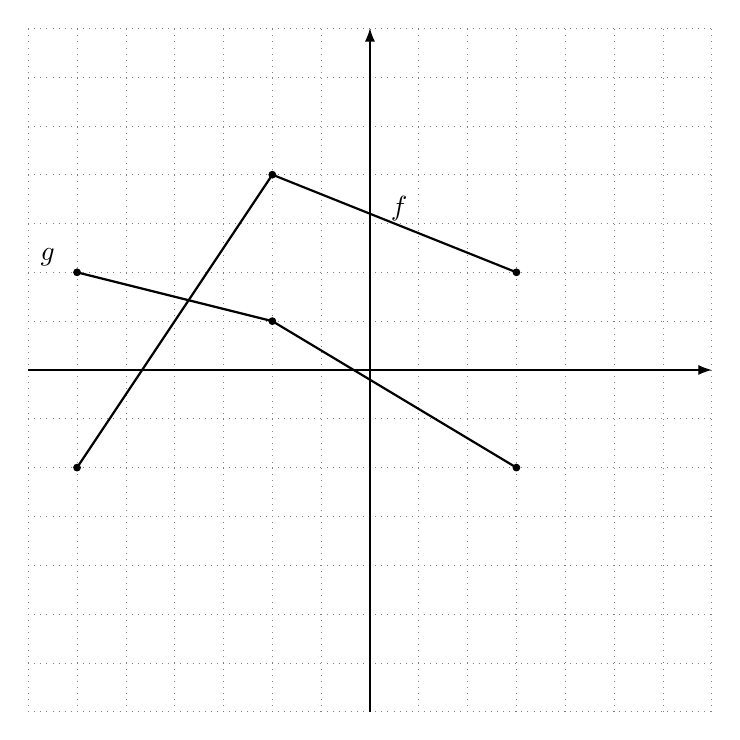
\begin{tikzpicture}[scale=0.62]
\draw[help lines, dotted] (-7,-7) grid (7,7);
\draw[-{Latex}] (-7,0) -- (7,0);
\draw[-{Latex}] (0,-7) -- (0,7);
\draw[thick] (-6,-2) -- (-2,4) -- (3,2);
\fill (-6,-2) circle (0.08);
\fill (-2,4) circle (0.08);
\fill (3,2) circle (0.08);
\node at (0.6,3.3) {$f$};
\draw[thick] (-6,2) -- (-2,1) -- (3,-2);
\fill (-6,2) circle (0.08);
\fill (-2,1) circle (0.08);
\fill (3,-2) circle (0.08);
\node at (-6.6,2.3) {$g$};
\end{tikzpicture}
\end{center}

 

\begin{solutionbox}
As before: $f(-6)=-2$, $f(-2)=4$, $f(3)=2$, and $g(-6)=2$, $g(-2)=1$, $g(3)=-2$.

\textbf{(a)}

\[
(g\circ f)(-6)=g(f(-6))=g(-2)=1.
\]

\textbf{(b)}

\[
(f\circ g)(3)=f(g(3))=f(-2)=4.
\]
\end{solutionbox}

  

\begin{friendlyex}{}
Using the table below, find the following.

\[
\begin{array}{c|ccccc}
x & 0 & 2 & 3 & 4 & 5 \\ \hline
f(x) & 3 & 1 & 2 & 5 & 0 \\
g(x) & 5 & 7 & 4 & 3 & 1
\end{array}
\]

\begin{multicols}{2}
\begin{itemize}
    \item[(a)] $(g-f)(2)$
    \item[(b)] $(f+g)(0)$
    \item[(c)] $(fg)(3)$
    \item[(d)] $\left(\dfrac{g}{f}\right)(5)$
    \item[(e)] $(g\circ f)(4)$
    \item[(f)] $(f\circ g)(4)$
    \item[(g)] $(f\circ g)(2)$
\end{itemize}
\end{multicols}
\end{friendlyex}

 

\begin{solutionbox}
\textbf{(a)} $(g-f)(2)=g(2)-f(2)=7-1=6$.

\textbf{(b)} $(f+g)(0)=f(0)+g(0)=3+5=8$.

\textbf{(c)} $(fg)(3)=f(3)\cdot g(3)=2\cdot 4=8$.

\textbf{(d)} $\left(\dfrac{g}{f}\right)(5)=\dfrac{g(5)}{f(5)}=\dfrac{1}{0}$, which is \textbf{undefined} --- $f(5)=0$, so we cannot divide by it.

\textbf{(e)} $(g\circ f)(4)=g(f(4))=g(5)=1$.

\textbf{(f)} $(f\circ g)(4)=f(g(4))=f(3)=2$.

\textbf{(g)} $(f\circ g)(2)=f(g(2))=f(7)$. But $x=7$ does not appear in the table, so $f(7)$ is \textbf{not determined} by the given information --- this composition cannot be computed from the table.
\end{solutionbox}

  

\begin{friendlyex}{}
Suppose $f(x)$ gives the miles that can be driven in $x$ hours, and $g(y)$ gives the gallons of gas used driving $y$ miles. What does the composite function $(g\circ f)(x)$ give? Is $f\circ g$ a meaningful composition? Explain why.
\end{friendlyex}

 

\begin{solutionbox}
$(g\circ f)(x)=g(f(x))$: first find $f(x)$, the miles driven in $x$ hours; then apply $g$ to that many miles, giving the gallons of gas used. So $(g\circ f)(x)$ gives \textbf{the gallons of gas used after driving for $x$ hours}. This is meaningful, since the output of $f$ (miles) matches exactly what $g$ expects as an input (miles).

$f\circ g$ is \textbf{not} meaningful: $g(y)$ outputs gallons of gas, but $f$ expects an input in hours. Feeding a number of gallons into $f$ does not correspond to any real quantity --- the output type of $g$ does not match the input type of $f$.
\end{solutionbox}

  

\section*{Summary}

\begin{friendlyrule}{Key Ideas}
\begin{itemize}
    \item $(f+g)(x)$, $(f-g)(x)$, $(fg)(x)$ combine $f$ and $g$ pointwise; their domain is the overlap of the domains of $f$ and $g$.
    \item $\left(\dfrac{f}{g}\right)(x)$ also requires $g(x)\neq 0$.
    \item $(g\circ f)(x)=g(f(x))$ means $f$ acts first, then $g$ acts on the result. Composition order matters: usually $f\circ g\neq g\circ f$.
    \item $(f\circ g)(x)$ and $(fg)(x)$ are different operations --- composition versus product.
    \item A composition is only meaningful when the output type of the inner function matches the expected input of the outer function.
\end{itemize}
\end{friendlyrule}

\end{document}
